\documentclass[tikz,border=10pt]{standalone}
\usepackage{tikz}
\usetikzlibrary{arrows.meta,positioning,calc,backgrounds,fit,shapes.geometric}
\usepackage[scaled=0.92]{helvet}
\renewcommand{\familydefault}{\sfdefault}
\usepackage{amsmath,amssymb}
\definecolor{ink}{HTML}{262624}
\definecolor{mute}{HTML}{8A8984}
\definecolor{line}{HTML}{BDBBB5}
\definecolor{acc}{HTML}{2A78D6}
\definecolor{accbg}{HTML}{F1F6FD}
\tikzset{
  >={Latex[length=2.2mm]},
  every node/.style={text=ink},
  b/.style={draw=line, fill=white, rounded corners=2pt, align=center, inner sep=6pt,
            minimum height=10mm, text width=#1, font=\small},
  b/.default=40mm,
  a/.style={b=#1, draw=acc, fill=accbg},
  a/.default=40mm,
  t/.style={font=\footnotesize, text=mute, align=center},
  e/.style={->, draw=mute, line width=0.6pt},
  ea/.style={->, draw=acc, line width=0.9pt},
  eh/.style={->, draw=acc, line width=0.9pt, dash pattern=on 3pt off 2pt},
}

\begin{document}
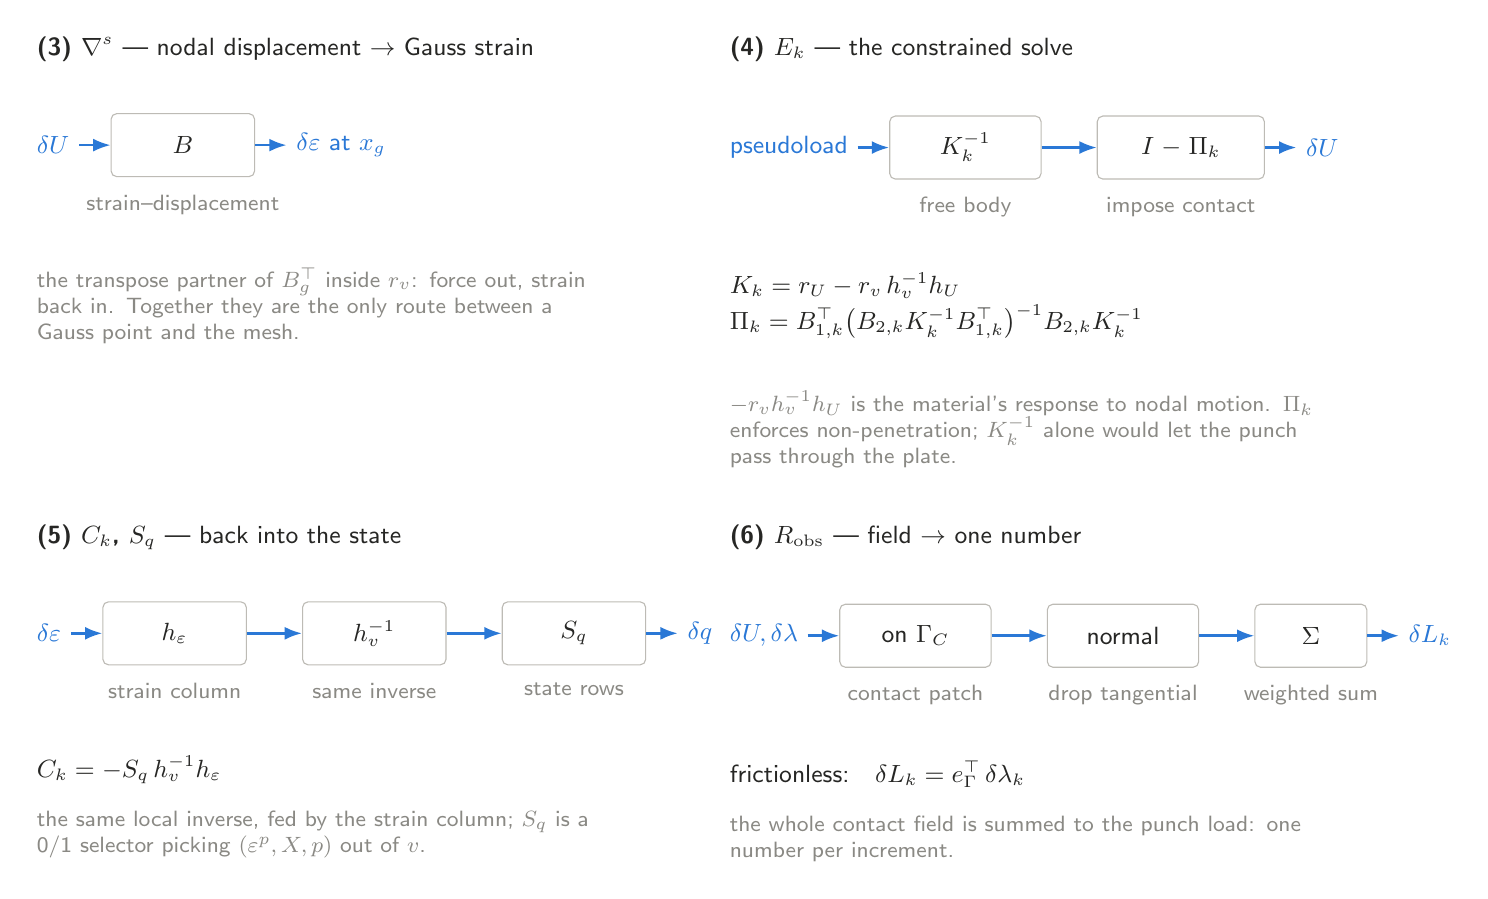
\begin{tikzpicture}
\tikzset{s/.style={b=#1, minimum height=8mm}, s/.default=14mm}
% (3) kinematics
\node[anchor=north west, font=\small\bfseries] (t3) at (0,0) {(3)\ $\nabla^s$ \textmd{--- nodal displacement $\to$ Gauss strain}};
\node[below=7mm of t3.south west, anchor=north west, font=\small, text=acc] (u3) {$\delta U$};
\node[s, right=4mm of u3] (B) {$B$};
\node[right=4mm of B, font=\small, text=acc] (e3) {$\delta\varepsilon$ at $x_g$};
\draw[ea] (u3) -- (B); \draw[ea] (B) -- (e3);
\node[below=1mm of B, t] {strain--displacement};
\node[below=12mm of u3.south west, anchor=north west, t, align=left, text width=70mm] {the transpose partner of $B_g^{\top}$ inside $r_v$: force out, strain back in. Together they are the only route between a Gauss point and the mesh.};
% (4) constrained solve
\begin{scope}[shift={(88mm,0)}]
\node[anchor=north west, font=\small\bfseries] (t4) at (0,0) {(4)\ $E_k$ \textmd{--- the constrained solve}};
\node[below=7mm of t4.south west, anchor=north west, font=\small, text=acc] (p4) {pseudoload};
\node[s=15mm, right=4mm of p4] (Ki) {$K_k^{-1}$};
\node[s=17mm, right=7mm of Ki] (Pi) {$I-\Pi_k$};
\node[right=4mm of Pi, font=\small, text=acc] (u4) {$\delta U$};
\draw[ea] (p4) -- (Ki); \draw[ea] (Ki) -- (Pi); \draw[ea] (Pi) -- (u4);
\node[below=1mm of Ki, t] {free body}; \node[below=1mm of Pi, t] {impose contact};
\node[below=12mm of p4.south west, anchor=north west, font=\small, align=left] {%
$K_k = r_U - r_v\,h_v^{-1}h_U$\\[2pt]
$\Pi_k = B_{1,k}^{\top}\big(B_{2,k}K_k^{-1}B_{1,k}^{\top}\big)^{-1}B_{2,k}K_k^{-1}$};
\node[below=27mm of p4.south west, anchor=north west, t, align=left, text width=78mm] {$-r_v h_v^{-1} h_U$ is the material's response to nodal motion. $\Pi_k$ enforces non-penetration; $K_k^{-1}$ alone would let the punch pass through the plate.};
\end{scope}
% (5) back into the state
\begin{scope}[shift={(0,-62mm)}]
\node[anchor=north west, font=\small\bfseries] (t5) at (0,0) {(5)\ $C_k$, $S_q$ \textmd{--- back into the state}};
\node[below=7mm of t5.south west, anchor=north west, font=\small, text=acc] (e5) {$\delta\varepsilon$};
\node[s, right=4mm of e5] (he) {$h_\varepsilon$};
\node[s, right=7mm of he] (hv) {$h_v^{-1}$};
\node[s, right=7mm of hv] (Sq) {$S_q$};
\node[right=4mm of Sq, font=\small, text=acc] (q5) {$\delta q$};
\draw[ea] (e5) -- (he); \draw[ea] (he) -- (hv); \draw[ea] (hv) -- (Sq); \draw[ea] (Sq) -- (q5);
\node[below=1mm of he, t] {strain column}; \node[below=1mm of hv, t] {same inverse}; \node[below=1mm of Sq, t] {state rows};
\node[below=12mm of e5.south west, anchor=north west, font=\small] {$C_k = -S_q\,h_v^{-1}h_\varepsilon$};
\node[below=19mm of e5.south west, anchor=north west, t, align=left, text width=74mm] {the same local inverse, fed by the strain column; $S_q$ is a 0/1 selector picking $(\varepsilon^p, X, p)$ out of $v$.};
\end{scope}
% (6) readout
\begin{scope}[shift={(88mm,-62mm)}]
\node[anchor=north west, font=\small\bfseries] (t6) at (0,0) {(6)\ $R_{\rm obs}$ \textmd{--- field $\to$ one number}};
\node[below=7mm of t6.south west, anchor=north west, font=\small, text=acc] (u6) {$\delta U,\delta\lambda$};
\node[s=15mm, right=4mm of u6] (gc) {on $\Gamma_C$};
\node[s=15mm, right=7mm of gc] (nm) {normal};
\node[s=10mm, right=7mm of nm] (sm) {$\Sigma$};
\node[right=4mm of sm, font=\small, text=acc] (l6) {$\delta L_k$};
\draw[ea] (u6) -- (gc); \draw[ea] (gc) -- (nm); \draw[ea] (nm) -- (sm); \draw[ea] (sm) -- (l6);
\node[below=1mm of gc, t] {contact patch}; \node[below=1mm of nm, t] {drop tangential}; \node[below=1mm of sm, t] {weighted sum};
\node[below=12mm of u6.south west, anchor=north west, font=\small, align=left] {%
frictionless:\quad $\delta L_k = e_{\Gamma}^{\top}\,\delta\lambda_k$};
\node[below=19mm of u6.south west, anchor=north west, t, align=left, text width=78mm] {the whole contact field is summed to the punch load: one number per increment.};
\end{scope}
\end{tikzpicture}
\end{document}
